\section{原理}

\subsection{超音波探傷法の原理}
超音波とは人間の耳に聞こえない音であり,周波数が20kHz以上の音波を指す.超音波の送受信は圧電素子により行われる.送受信の役目を担う素子を振動子と呼び,振動子に吸音材と保護版を貼り付け,ケース格納したものを探触子と呼ぶ.探触子を試験体に押し付けるだけでは,超音波はほとんど入射しないため,接触媒質を介して入射させる必要がある.本実験では直接接触法と水浸法の2種類を用いた(図\ref{fig:カップリング}).探傷方法はパルス波を用いたパルス反射法である(図\ref{fig:パルス反射法}).図\ref{fig:パルス反射法}のように反射したエコーから欠陥の情報を得ることができる.エコーの往復時間が欠陥の位置に対応し,エコーの高さが欠陥の寸法に対応する.

\begin{figure}[htbp]
    \centering %中央揃え
    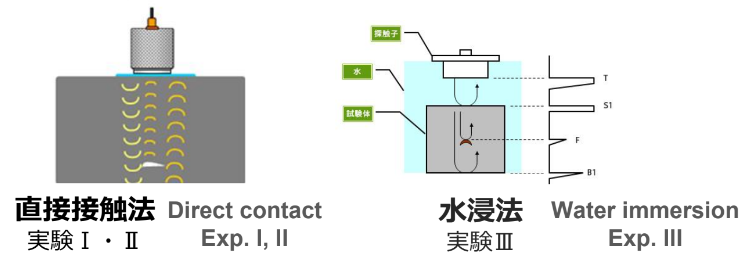
\includegraphics[width=100truemm,clip]{fig/fig_測定方式.png}
    \caption{Coupling Methods in Ultrasonic Flaw Detection.}
    \label{fig:カップリング}
\end{figure}

\begin{figure}[htbp]
    \centering %中央揃え
    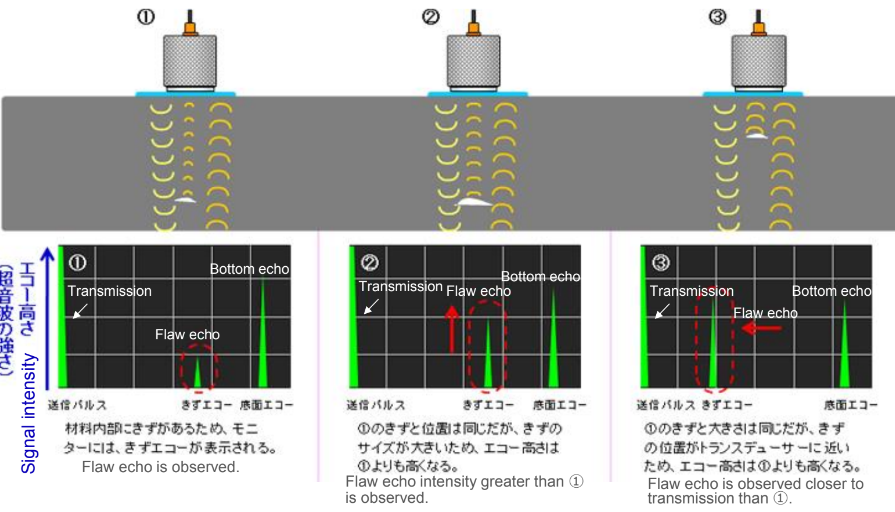
\includegraphics[width=100truemm,clip]{fig/fig_探傷法.png}
    \caption{Pulse echo technique.}
    \label{fig:パルス反射法}
\end{figure}

\subsection{AVG線図を用いた欠陥エコーの評価}
同じ大きさの欠陥でも,探傷面から欠陥までの距離が異なれば,超音波の広がりと減衰によって欠陥エコー高さは異なる.このため,欠陥の大きさを評価するためにAVG線図が用いられる.図\ref{fig:AVG線図}は一般化されたAVG線図であり,規準化されたエコー高さ(縦軸)と音波路程(横軸)との関係を異なる直径の円形平面傷に対して描いたグラフである.欠陥の大きさも振動子の直径によって規準化されている.

\begin{figure}[htbp]
    \centering %中央揃え
    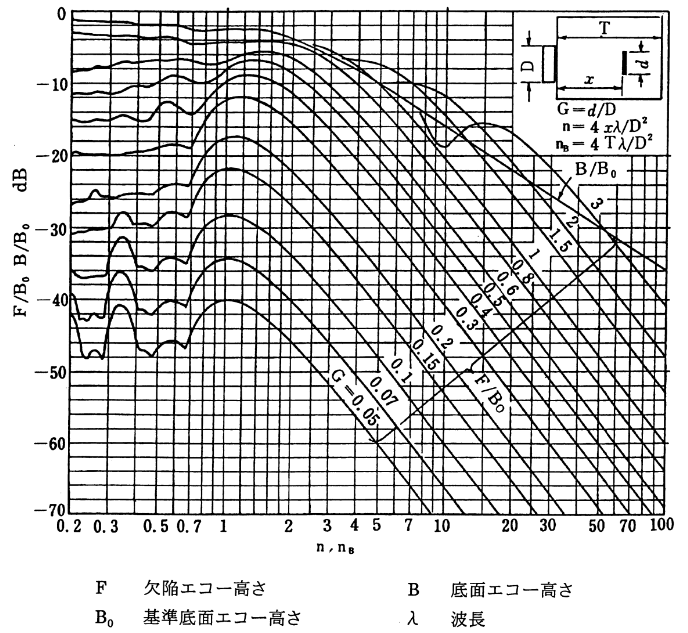
\includegraphics[width=100truemm,clip]{fig/AVG線図.png}
    \caption{AVG diagram for circular planar wounds.}
    \label{fig:AVG線図}
\end{figure}
